% STATUS: ACTIVE -- first-order gain model: the observability matrix, what it shows, and solving it (average, speed).
% ======================================================
% Compile: xelatex 0927_obs_first_order_v1.tex   (from reference/eq17_analysis/derivation/)
% Notation: 0921_5state_noap_simple.tex (teacher chain) with delta a removed. Every symbol is defined where it first appears.
% Sections: 1 model | 2 the matrix | 3 what it shows | 4 solving the matrix equation (average, speed) | 5 Kalman filter -> 4.7 | 6 two tracks per step, the estimate unrolled.
% Figure: fig_noap_descent_td5_td50.png (test_script/scratch/plot_5state_noap_descent_td5_td50.m;
%   runs ladder_ramp16_Td5_lf1_o1.mat, ladder_ramp16_Td50_lf1_s{1..5}_o1.mat; descent drawn, 0.5 s holds still in the runs). 
% Equations only (derivation-workflow rule 10).
% ======================================================
\documentclass[11pt,a4paper]{ctexart}
\usepackage[fleqn]{amsmath}
\usepackage{amssymb,bm}
\usepackage{graphicx}
\graphicspath{{figures/}}
\setlength{\mathindent}{0pt}
\usepackage{geometry}
\geometry{margin=2.2cm}
\setlength{\parindent}{0pt}
\setlength{\parskip}{0.2em}
\setlength{\abovedisplayskip}{6pt}
\setlength{\belowdisplayskip}{6pt}
\setlength{\abovedisplayshortskip}{6pt}
\setlength{\belowdisplayshortskip}{6pt}
\newcommand{\lc}{\lambda_c}
\newcommand{\hd}[1]{\par\bigskip\noindent\underline{\textbf{#1}}}
\pagestyle{plain}

\begin{document}

\begin{center}\textbf{\large First-order gain model: observability matrix}\end{center}

%======================================================================
\section{Model}

\hd{State equation}
\[
\begin{aligned}
\delta x_1[k+1] &= \delta x_2[k] \\
\delta x_2[k+1] &= \delta x_3[k] \\
\delta x_3[k+1] &= \lc \cdot \delta x_3[k] - F_{dx}[k]\cdot e_{a_x}[k] - \varepsilon[k] \\
a_x[k+1] &= a_x[k]
\end{aligned}
\]
\[
F_{dx}[k] = f_{dx}[k] + (1-\lc)\textstyle\sum_{i=1}^{d} f_{dx}[k-i] \;\approx\; \big(1 + (1-\lc)d\big)\,\dfrac{\Delta x_d[k]}{\hat a_x[k]} \qquad (\text{constant velocity})
\]

\hd{Output equation}
\[
\begin{aligned}
y_1[k] &= \delta x_1[k] + n_x[k], \qquad R_1 = \mathrm{Var}(n_x) \\
y_2[k] &= a_x[k] + n_a[k], \qquad\;\; R_2 = \mathrm{Var}(n_a)
\end{aligned}
\]

\hd{Estimation error and output error}
\[
\mathbf{e}[k] = \begin{bmatrix} e_{\delta x_1}[k] \\ e_{\delta x_2}[k] \\ e_{\delta x_3}[k] \\ e_{a_x}[k] \end{bmatrix}
= \begin{bmatrix} \delta x_1[k] - \delta\hat x_1[k] \\ \delta x_2[k] - \delta\hat x_2[k] \\ \delta x_3[k] - \delta\hat x_3[k] \\ a_x[k] - \hat a_x[k] \end{bmatrix},
\qquad
\begin{aligned}
e_{y_1}[k] &= y_1[k] - \delta\hat x_1[k] = e_{\delta x_1}[k] + n_x[k] \\
e_{y_2}[k] &= y_2[k] - \hat a_x[k] = e_{a_x}[k] + n_a[k]
\end{aligned}
\]

\hd{Error propagation (no noise)}
\[
\mathbf{e}[k+1] = \mathbf{F}_e[k]\,\mathbf{e}[k], \quad
\mathbf{F}_e[k] =
\begin{bmatrix}
0 & 1 & 0 & 0 \\
0 & 0 & 1 & 0 \\
0 & 0 & \lc & -F_{dx}[k] \\
0 & 0 & 0 & 1
\end{bmatrix};
\qquad
\begin{bmatrix} e_{y_1}[k] \\ e_{y_2}[k] \end{bmatrix} = \mathbf{H}\,\mathbf{e}[k], \quad
\mathbf{H} =
\begin{bmatrix}
1 & 0 & 0 & 0 \\
0 & 0 & 0 & 1
\end{bmatrix}
\]

%======================================================================
\section{Observability matrix}

\hd{Errors at step $k_0$, output errors $j$ steps later}
\[
\begin{bmatrix} e_{y_1}[k_0+j] \\ e_{y_2}[k_0+j] \end{bmatrix}
= \mathbf{H}\,\mathbf{F}_e[k_0+j-1]\cdots\mathbf{F}_e[k_0]\;\mathbf{e}[k_0]
\]

\hd{The matrix}
\[
\begin{bmatrix} e_{y_1}[k_0] \\ e_{y_2}[k_0] \\[0.3ex] e_{y_1}[k_0+1] \\ e_{y_2}[k_0+1] \\[0.3ex] e_{y_1}[k_0+2] \\ e_{y_2}[k_0+2] \\[0.3ex] e_{y_1}[k_0+3] \\ e_{y_2}[k_0+3] \\[0.3ex] e_{y_1}[k_0+4] \\ e_{y_2}[k_0+4] \\ \vdots \\ e_{y_1}[k_0+j] \\ e_{y_2}[k_0+j] \end{bmatrix}
=
\underbrace{\begin{bmatrix}
1 & 0 & 0 & 0 \\
0 & 0 & 0 & 1 \\[0.3ex]
0 & 1 & 0 & 0 \\
0 & 0 & 0 & 1 \\[0.3ex]
0 & 0 & 1 & 0 \\
0 & 0 & 0 & 1 \\[0.3ex]
0 & 0 & \lc & -F_{dx}[k_0] \\
0 & 0 & 0 & 1 \\[0.3ex]
0 & 0 & \lc^2 & -\lc F_{dx}[k_0] - F_{dx}[k_0+1] \\
0 & 0 & 0 & 1 \\
\vdots & \vdots & \vdots & \vdots \\
0 & 0 & \lc^{\,j-2} & -\sum_{i=0}^{j-3}\lc^{\,j-3-i}F_{dx}[k_0+i] \\
0 & 0 & 0 & 1
\end{bmatrix}}_{\mathbf{O}(k_0)}
\begin{bmatrix} e_{\delta x_1}[k_0] \\ e_{\delta x_2}[k_0] \\ e_{\delta x_3}[k_0] \\ e_{a_x}[k_0] \end{bmatrix}
\]

\hd{The four columns ($F_{dx}$ constant)}
\[
\begin{aligned}
e_{\delta x_1}:&\quad y_1:\; 1, 0, 0, 0, \dots & y_2:&\; 0, 0, 0, \dots \\
e_{\delta x_2}:&\quad y_1:\; 0, 1, 0, 0, \dots & y_2:&\; 0, 0, 0, \dots \\
e_{\delta x_3}:&\quad y_1:\; 0, 0, 1, \lc, \lc^2, \dots, \lc^{\,j-2} \to 0 & y_2:&\; 0, 0, 0, \dots \\
e_{a_x}:&\quad y_1:\; 0, 0, 0, -F_{dx}, -F_{dx}(1+\lc), \dots \to -\dfrac{F_{dx}}{1-\lc} & y_2:&\; 1, 1, 1, \dots
\end{aligned}
\]

%======================================================================
\section{What the matrix shows}

\hd{$y_2$ sees only the gain error, the same at every step}
\[
e_{y_2}[k_0+j] = 1\cdot e_{a_x}[k_0] \qquad \text{for every } j
\]

\hd{$y_1$ sees the gain error only through $F_{dx}$}
\[
e_{y_1}[k_0+j]\Big|_{e_{a_x}} \;\to\; -\frac{F_{dx}}{1-\lc}\,e_{a_x}[k_0]
= -\frac{1 + (1-\lc)d}{1-\lc}\cdot\frac{\Delta x_d}{\hat a_x}\,e_{a_x}[k_0]
\]
\[
\text{hold: } \Delta x_d = 0 \;\Rightarrow\; e_{y_1}\Big|_{e_{a_x}} = 0; \qquad
\text{faster } (\Delta x_d \uparrow) \text{ or nearer the wall } (\hat a_x \downarrow) \;\Rightarrow\; \Big|e_{y_1}\big|_{e_{a_x}}\Big| \uparrow
\]

\hd{Where $T_d$ enters}
\[
\begin{aligned}
&R = \text{particle radius}, \qquad T_s = \text{sampling period}, \qquad T_d = \text{descent time} \\
&h_0,\, h_b = \text{start and bottom height of the descent, in units of } R \\
&\Delta x_d = \frac{\text{distance}}{\text{number of steps}} = \frac{(h_0 - h_b)\,R}{T_d / T_s} \\
&y_1 \text{ entry of } e_{a_x} \propto \frac{1}{T_d\,\hat a_x}, \qquad y_2 \text{ entry of } e_{a_x} = 1
\end{aligned}
\]

%======================================================================
\clearpage
\section{Solving the matrix equation}

\hd{4.1 The $y_2$ rows written out ($\hat a_x$ stays at $\hat a_x[k_0]$ because $\hat a_x[k+1] = \hat a_x[k]$)}
\[
\begin{aligned}
e_{y_2}[k_0+1] &= y_2[k_0+1] - \hat a_x[k_0] = e_{a_x}[k_0] + n_a[k_0+1] \\
e_{y_2}[k_0+2] &= y_2[k_0+2] - \hat a_x[k_0] = e_{a_x}[k_0] + n_a[k_0+2] \\
&\;\;\vdots \\
e_{y_2}[k_0+N] &= y_2[k_0+N] - \hat a_x[k_0] = e_{a_x}[k_0] + n_a[k_0+N]
\end{aligned}
\]

\hd{4.2 One number $e$ that fits all $N$ equations best}
\[
\begin{aligned}
\text{minimize}\quad & \sum_{j=1}^{N}\big(e_{y_2}[k_0+j] - e\big)^2 \\
\frac{d}{de}:\quad & -2\sum_{j=1}^{N}\big(e_{y_2}[k_0+j] - e\big) = 0 \\
& \hat e_{a_x}[k_0] = \frac{1}{N}\sum_{j=1}^{N} e_{y_2}[k_0+j]
\end{aligned}
\]

\hd{4.3 Back to the gain}
\[
\begin{aligned}
\hat a_x[k_0] + \hat e_{a_x}[k_0]
&= \hat a_x[k_0] + \frac{1}{N}\sum_{j=1}^{N}\big(y_2[k_0+j] - \hat a_x[k_0]\big) \\
&= \frac{1}{N}\sum_{j=1}^{N} y_2[k_0+j] \\
&= \frac{1}{N}\sum_{j=1}^{N} a_x[k_0+j] + \frac{1}{N}\sum_{j=1}^{N} n_a[k_0+j]
\qquad \big(y_2[k_0+j] = a_x[k_0+j] + n_a[k_0+j]\big)
\end{aligned}
\]

\hd{4.4 A $y_1$ row turned into a reading of $e_{a_x}$ (position errors known)}
\[
\begin{aligned}
e_{y_1}[k_0+j] &\approx -\frac{F_{dx}}{1-\lc}\,e_{a_x}[k_0] + n_x[k_0+j] \\
-\frac{1-\lc}{F_{dx}}\,e_{y_1}[k_0+j] &\approx e_{a_x}[k_0] - \frac{1-\lc}{F_{dx}}\,n_x[k_0+j],
\qquad \mathrm{Var} = \left(\frac{1-\lc}{F_{dx}}\right)^{2} R_1
\end{aligned}
\]

\hd{4.5 Readings with different noise: weight = $1/\mathrm{Var}$}
\[
\begin{aligned}
y_2 \text{ row:}&\quad \frac{1}{R_2} \\
y_1 \text{ row:}&\quad \frac{1}{R_1}\left(\frac{F_{dx}}{1-\lc}\right)^{2}
= \frac{1}{R_1}\left(\frac{1+(1-\lc)d}{1-\lc}\cdot\frac{\Delta x_d}{\hat a_x}\right)^{2}
\end{aligned}
\]

\hd{4.6 The gain moves, both rows: weighted average}
\[
\boxed{\;
\hat a_x[k_0] + \hat e_{a_x}[k_0] \approx
\frac{\displaystyle\sum_{j=1}^{N} w_j\, a_x[k_0+j]}{\displaystyle\sum_{j=1}^{N} w_j},
\qquad
w_j = \frac{1}{R_2} + \frac{1}{R_1}\Big(\frac{F_{dx}[k_0+j]}{1-\lc}\Big)^{2}
\;}
\]

\hd{4.7 What the figure computes (weights read from the filter, initial estimate included)}
\[
\boxed{\;
\begin{aligned}
\hat a_x[k] &= \frac{\dfrac{1}{P_{aa}[0]}\,\hat a_x[0] + \displaystyle\sum_{j=1}^{k} w_j\, a_x[j]}{\dfrac{1}{P_{aa}[0]} + \displaystyle\sum_{j=1}^{k} w_j} \\[1ex]
w_j &= \frac{1}{P_{aa}[j]} - \frac{1}{P_{aa}[j-1]} \;\approx\; \frac{1}{R_2} + \frac{1}{R_1}\Big(\frac{F_{dx}[j]}{1-\lc}\Big)^{2}
\end{aligned}
\;}
\qquad
\begin{aligned}
&P_{aa} = \text{variance of the gain estimate} \\
&P_{aa}[0] = \text{its initial value}
\end{aligned}
\]

%======================================================================
\clearpage
\section{Kalman filter: where 4.7 comes from}

\hd{5.1 Kalman filter, every step}
\[
\begin{aligned}
\hat{\mathbf{x}}^f[k] &= \text{state equation applied to } \hat{\mathbf{x}}[k-1] \\
\mathbf{P}^f[k] &= \mathbf{F}_e[k-1]\,\mathbf{P}[k-1]\,\mathbf{F}_e^T[k-1] + \mathbf{Q} \\
\mathbf{L}[k] &= \mathbf{P}^f[k]\,\mathbf{H}^T\big(\mathbf{H}\,\mathbf{P}^f[k]\,\mathbf{H}^T + \mathbf{R}\big)^{-1} \\
\hat{\mathbf{x}}[k] &= \hat{\mathbf{x}}^f[k] + \mathbf{L}[k]\big(\mathbf{y}[k] - \hat{\mathbf{y}}[k]\big), \qquad \hat{\mathbf{y}}[k] = \mathbf{H}\,\hat{\mathbf{x}}^f[k] \\
\mathbf{P}[k] &= \big[\mathbf{I} - \mathbf{L}[k]\,\mathbf{H}\big]\,\mathbf{P}^f[k]
\end{aligned}
\]
\[
\mathbf{P} = \text{error covariance}, \qquad
\mathbf{Q} = \mathrm{diag}(0,\, 0,\, Q_{33},\, 0), \qquad
\mathbf{R} = \mathrm{diag}(R_1,\, R_2)
\]

\hd{5.2 The $a_x$ element, $y_2$ only}
\[
\begin{aligned}
\hat a_x^f[k] &= \hat a_x[k-1] \\
P^f_{aa}[k] &= P_{aa}[k-1] + Q_{44} = P_{aa}[k-1] \\
\ell_{42}[k] &= \frac{P^f_{aa}[k]}{P^f_{aa}[k] + R_2} \\
\hat a_x[k] &= \hat a_x^f[k] + \ell_{42}[k]\,\big(y_2[k] - \hat a_x^f[k]\big) \\
P_{aa}[k] &= \big(1 - \ell_{42}[k]\big)\,P^f_{aa}[k]
\end{aligned}
\]

\hd{5.3 $P_{aa}$ written as $1/P_{aa}$}
\[
\begin{aligned}
P_{aa}[k] &= \frac{R_2}{P_{aa}[k-1] + R_2}\,P_{aa}[k-1] \\
\frac{1}{P_{aa}[k]} &= \frac{P_{aa}[k-1] + R_2}{R_2\,P_{aa}[k-1]} = \frac{1}{P_{aa}[k-1]} + \frac{1}{R_2}
\end{aligned}
\]

\hd{5.4 $\hat a_x$ written as $\hat a_x / P_{aa}$}
\[
\begin{aligned}
\ell_{42}[k] &= \frac{P_{aa}[k-1]}{P_{aa}[k-1] + R_2} = \frac{P_{aa}[k]}{R_2}, \qquad
1 - \ell_{42}[k] = \frac{R_2}{P_{aa}[k-1] + R_2} = \frac{P_{aa}[k]}{P_{aa}[k-1]} \\
\hat a_x[k] &= \big(1 - \ell_{42}[k]\big)\,\hat a_x[k-1] + \ell_{42}[k]\,y_2[k]
= P_{aa}[k]\left(\frac{\hat a_x[k-1]}{P_{aa}[k-1]} + \frac{y_2[k]}{R_2}\right) \\
\frac{\hat a_x[k]}{P_{aa}[k]} &= \frac{\hat a_x[k-1]}{P_{aa}[k-1]} + \frac{y_2[k]}{R_2}
\end{aligned}
\]

\hd{5.5 Unroll from step $0$ to step $k$}
\[
\begin{aligned}
\frac{1}{P_{aa}[k]} &= \frac{1}{P_{aa}[0]} + \sum_{j=1}^{k}\frac{1}{R_2} \\
\frac{\hat a_x[k]}{P_{aa}[k]} &= \frac{\hat a_x[0]}{P_{aa}[0]} + \sum_{j=1}^{k}\frac{1}{R_2}\,y_2[j] \\
\hat a_x[k] &= \frac{\dfrac{1}{P_{aa}[0]}\,\hat a_x[0] + \sum_{j=1}^{k}\dfrac{1}{R_2}\,y_2[j]}{\dfrac{1}{P_{aa}[0]} + \sum_{j=1}^{k}\dfrac{1}{R_2}}
\\
&\text{= 4.7 with } w_j = \frac{1}{R_2} = \frac{1}{P_{aa}[j]} - \frac{1}{P_{aa}[j-1]}, \qquad y_2[j] = a_x[j] + n_a[j]
\end{aligned}
\]

\hd{5.6 $y_1$ added: the $e_{a_x}$ column of $\mathbf{O}$ is carried in $\mathbf{P}^f$}
\[
\begin{aligned}
P^f_{3a}[k] &= \lc\,P_{3a}[k-1] - F_{dx}\,P_{aa}[k-1], \qquad P^f_{2a}[k] = P_{3a}[k-1], \qquad P^f_{1a}[k] = P_{2a}[k-1] \\
P^f_{1a} &\to -\frac{F_{dx}}{1-\lc}\,P_{aa} \qquad (\text{the } y_1 \text{ entry of the } e_{a_x} \text{ column, times } P_{aa}) \\
\ell_{41}[k] &= \frac{P^f_{a1}[k]}{P^f_{11}[k] + R_1}, \qquad
\frac{1}{P_{aa}[k]} - \frac{1}{P_{aa}[k-1]} \approx \frac{1}{R_2} + \frac{1}{P^f_{11}[k] + R_1}\left(\frac{F_{dx}}{1-\lc}\right)^{2} = w_k
\end{aligned}
\]

%======================================================================
\clearpage
\section{One step, two tracks; the estimate unrolled}

\hd{6.1 Track 1: confidence and gain (no measurement value enters)}
\[
\begin{aligned}
P^f_{aa}[k] &= P_{aa}[k-1] + Q_{44} \\
\ell_{42}[k] &= \frac{P^f_{aa}[k]}{P^f_{aa}[k] + R_2} \\
P_{aa}[k] &= \big(1 - \ell_{42}[k]\big)\,P^f_{aa}[k]
\end{aligned}
\]

\hd{6.2 Track 2: estimate (the measurement enters here only)}
\[
\begin{aligned}
\hat a_x^f[k] &= \hat a_x[k-1] \\
e_{y_2}[k] &= y_2[k] - \hat a_x^f[k] \\
\hat a_x[k] &= \hat a_x^f[k] + \ell_{42}[k]\,e_{y_2}[k] = \big(1 - \ell_{42}[k]\big)\,\hat a_x[k-1] + \ell_{42}[k]\,y_2[k]
\end{aligned}
\]

\hd{6.3 Unroll track 2}
\[
\begin{aligned}
\hat a_x[1] &= (1-\ell_{42}[1])\,\hat a_x[0] + \ell_{42}[1]\,y_2[1] \\
\hat a_x[2] &= (1-\ell_{42}[2])(1-\ell_{42}[1])\,\hat a_x[0] + (1-\ell_{42}[2])\,\ell_{42}[1]\,y_2[1] + \ell_{42}[2]\,y_2[2] \\
\hat a_x[3] &= (1-\ell_{42}[3])(1-\ell_{42}[2])(1-\ell_{42}[1])\,\hat a_x[0] + (1-\ell_{42}[3])(1-\ell_{42}[2])\,\ell_{42}[1]\,y_2[1] \\
&\quad + (1-\ell_{42}[3])\,\ell_{42}[2]\,y_2[2] + \ell_{42}[3]\,y_2[3] \\
\hat a_x[k] &= c_{k,0}\,\hat a_x[0] + \sum_{j=1}^{k} c_{k,j}\,y_2[j], \qquad
c_{k,j} = \ell_{42}[j]\prod_{i=j+1}^{k}\big(1 - \ell_{42}[i]\big), \qquad
c_{k,0} + \sum_{j=1}^{k} c_{k,j} = 1
\end{aligned}
\]

\hd{6.4 $Q_{44} = 0$: every coefficient equal (average)}
\[
\begin{aligned}
\ell_{42}[i] &= \frac{1}{i + m}, \quad m = \frac{R_2}{P_{aa}[0]}, \qquad
1 - \ell_{42}[i] = \frac{i + m - 1}{i + m} \\
\prod_{i=j+1}^{k}\big(1 - \ell_{42}[i]\big) &= \frac{j + m}{j + m + 1}\cdot\frac{j + m + 1}{j + m + 2}\cdots\frac{k + m - 1}{k + m} = \frac{j + m}{k + m} \\
c_{k,j} &= \frac{1}{j + m}\cdot\frac{j + m}{k + m} = \frac{1}{k + m} \qquad (\text{same for every } j)
\end{aligned}
\]

\hd{6.5 $Q_{44} > 0$: coefficients shrink with age (forgetting)}
\[
\begin{aligned}
\ell_{42}[k] &\to \ell^{*} \approx \sqrt{Q_{44}/R_2} \qquad (Q_{44} \ll R_2) \\
c_{k,j} &\approx \ell^{*}\,\big(1 - \ell^{*}\big)^{\,k-j}, \qquad \text{memory} \approx \frac{1}{\ell^{*}} = \sqrt{R_2/Q_{44}} \text{ steps}
\end{aligned}
\]

\clearpage
\section*{Descent only, $T_d = 5$ s vs $50$ s: filter $\hat a_x$ (blue) vs the boxed formula of 4.7 (green dashed)}
\begin{center}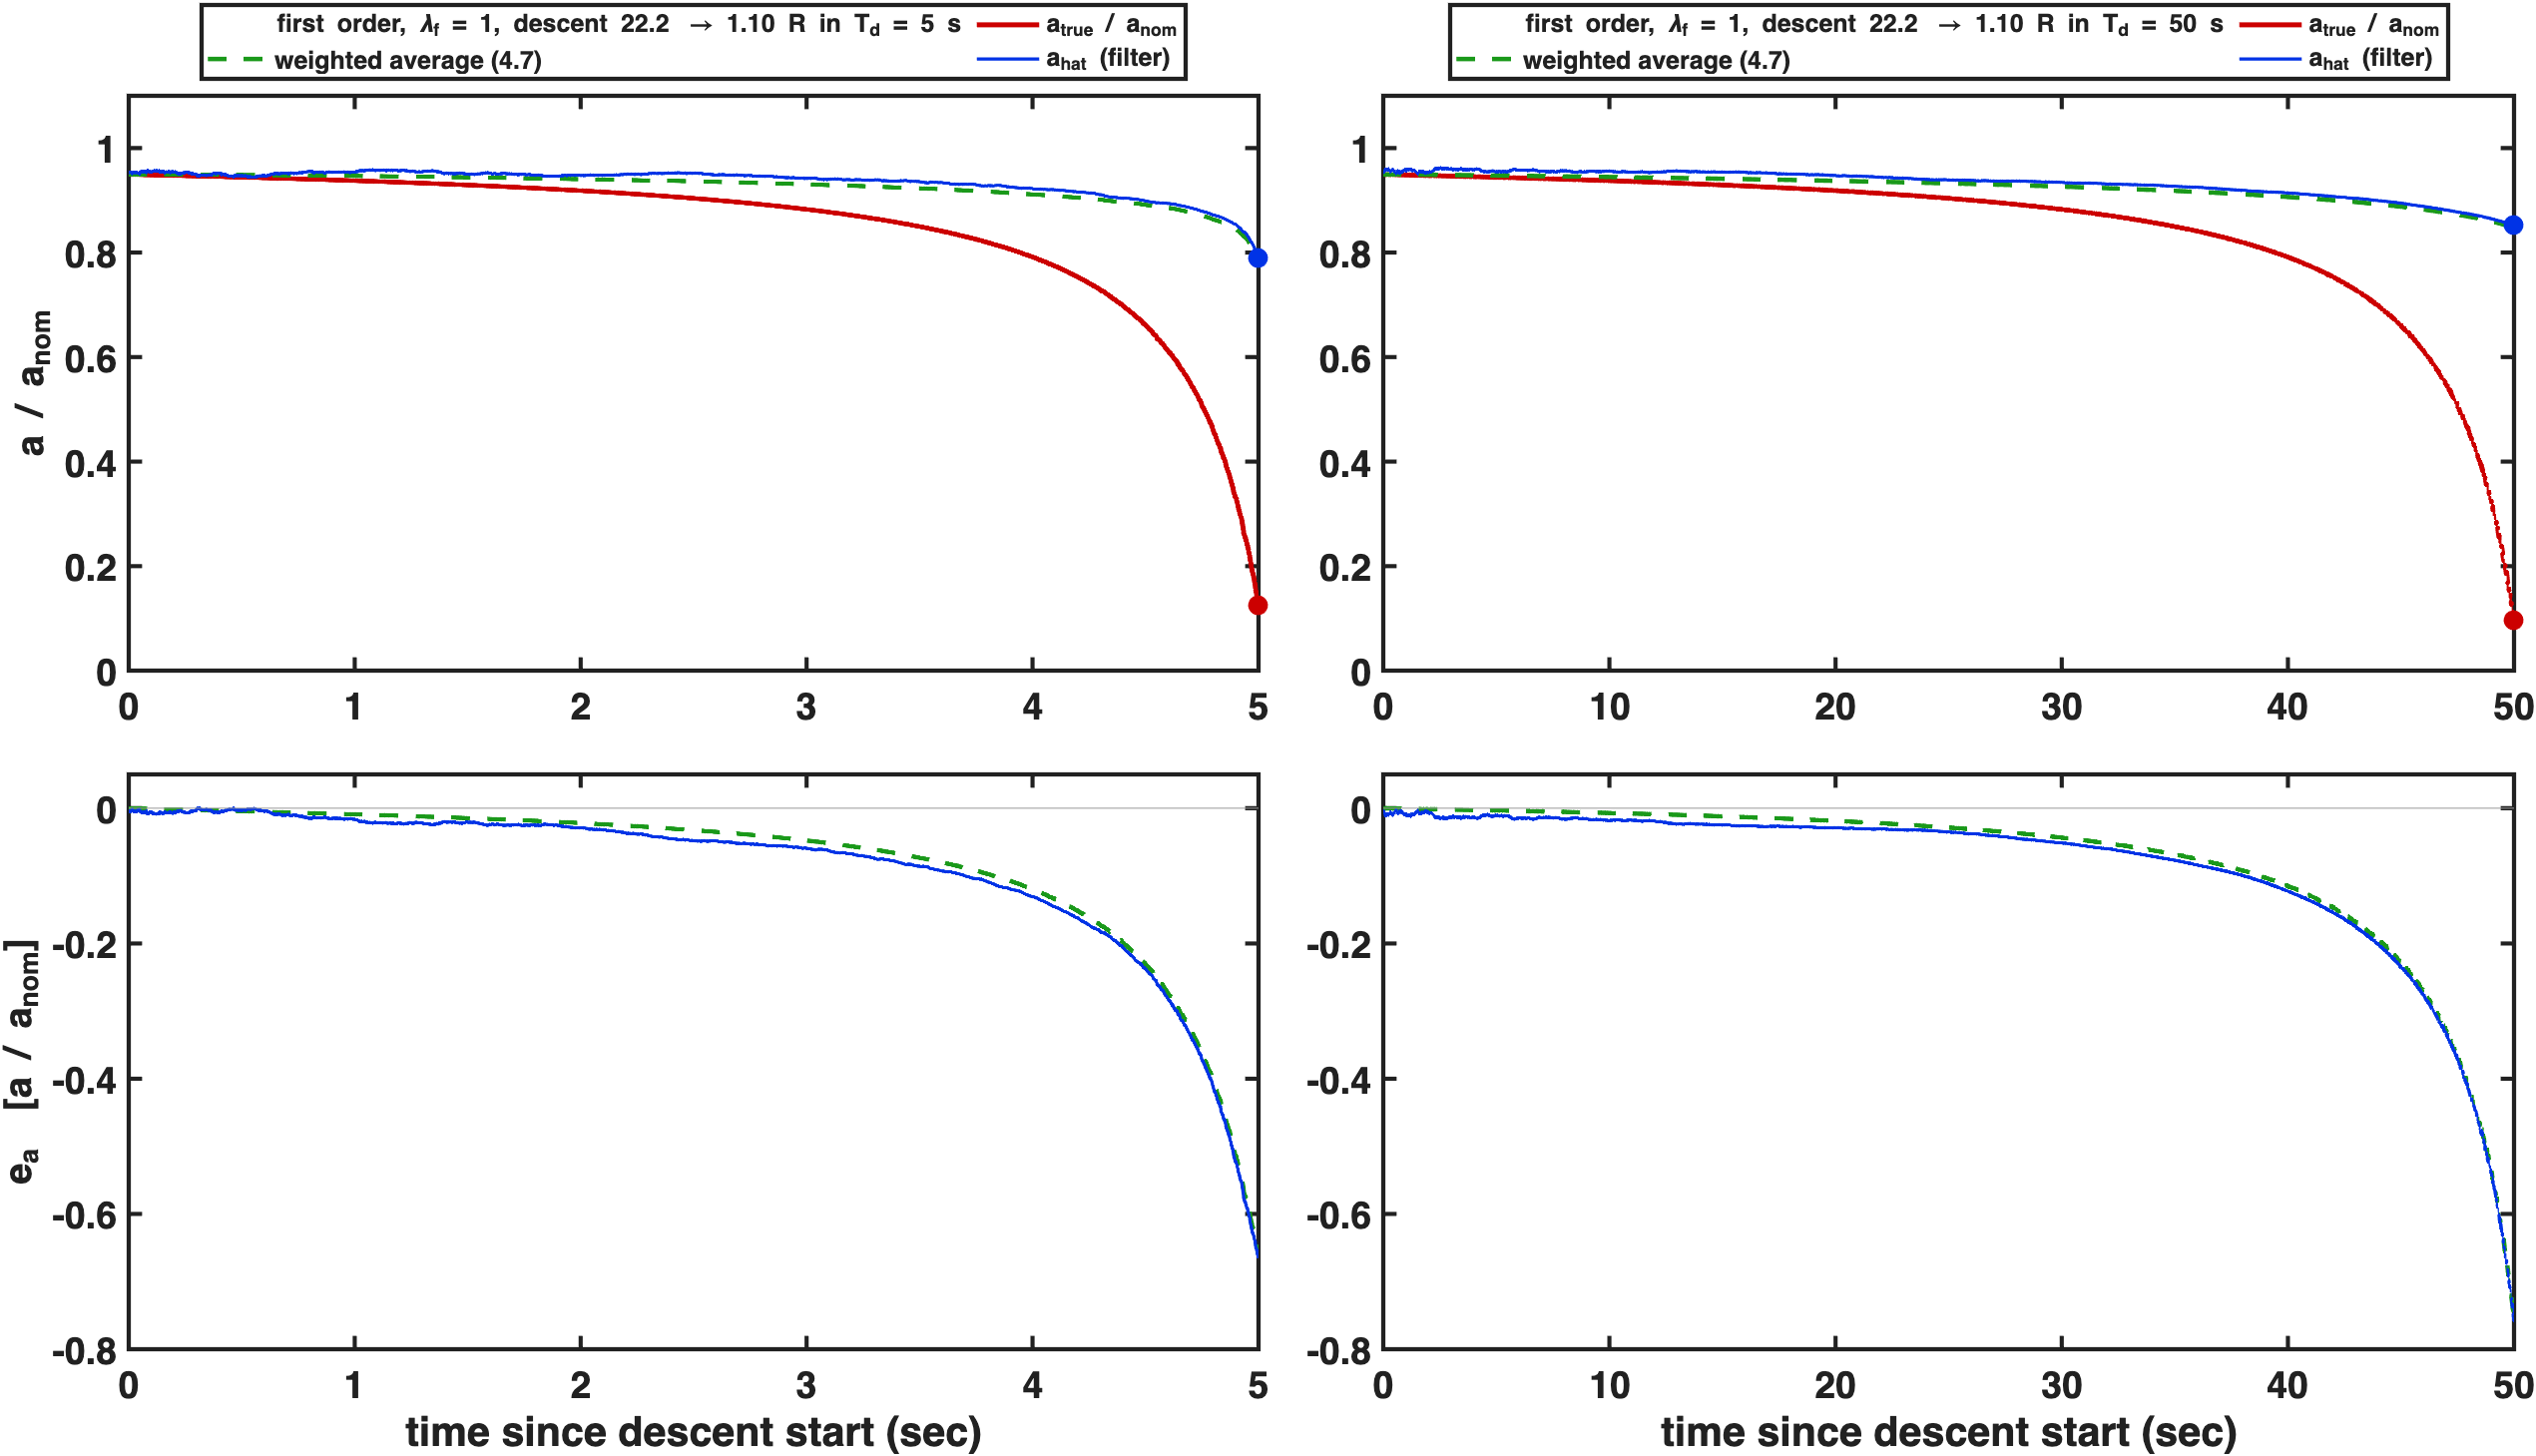
\includegraphics[width=\textwidth]{fig_noap_descent_td5_td50.png}\end{center}

\end{document}
